
%(BEGIN_QUESTION)
% Copyright 2012, Tony R. Kuphaldt, released under the Creative Commons Attribution License (v 1.0)
% This means you may do almost anything with this work of mine, so long as you give me proper credit

A 50 pound weight hangs by two strings, string {\bf A} pulling at an angle and string {\bf B} pulling horizontally.  The angle of string A is 60$^{o}$ from level (i.e. 30$^{o}$ from vertical).  Calculate the tension within each string:

$$\includegraphics[width=15.5cm]{i02587x01.eps}$$

\vskip 10pt

$F_{tension_A}$ = \underbar{\hskip 50pt} lbs

\vskip 10pt

$F_{tension_B}$ = \underbar{\hskip 50pt} lbs

\vskip 10pt

\underbar{file i02587}
%(END_QUESTION)





%(BEGIN_ANSWER)

In this system of forces, string {\bf A} exerts both a vertical and a horizontal force at the junction point of the three strings, just above the weight.  String {\bf B} only exerts a horizontal force at that point:

$$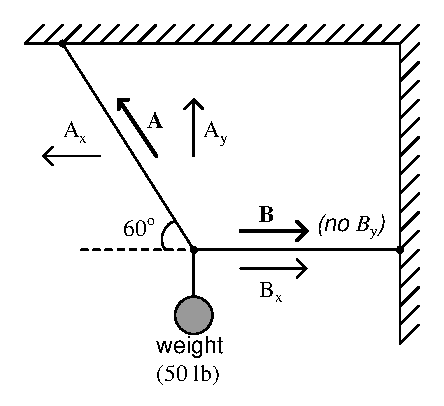
\includegraphics[width=15.5cm]{i02587x02.eps}$$

Because string A is the only one with a vertical force component, it must be doing all the work in suspending the 50 pound weight.  String B merely pulls laterally, and does not contribute to the effort of suspending the weight.  Therefore, if since we know $A_y$ is the only force component working to oppose the 50 pound vertical force of the weight, we can solve for A using trigonometry:

$$\includegraphics[width=15.5cm]{i02587x03.eps}$$

We have a right triangle with an opposite side length of 50 and an angle of 60$^{o}$.  To solve for the length of the hypotenuse:

\vskip 10pt

$F_{tension_A}$ = (50 lb)/(sin 60$^{o}$) = {\bf 57.735 lbs}

\vskip 10pt

So, string A must have a tension of 57.735 pounds.  That this figure is greater than 50 makes sense, because the angle of string A with respect to vertical makes it less efficient at opposing the force of the weight.  If the string were perfectly vertical, its tension would only have to be 50 pounds to suspend the weight, but since it is not perfectly vertical its tension must be more than that.

\vskip 10pt

Being angled, string A also exerts a horizontal force.  Since nothing in this system is moving, it must be in a condition of translational equilibrium, so the horizontal component of tension A (known as $A_x$) must be opposed by another force.  This other force is the tension of string B.  We may calculate $A_x$ (and, consequently, B as well), by using trigonometry again:

\vskip 10pt

$F_{tension_B} = A_x$ = (57.735 lb)(cos 60$^{o}$) = {\bf 28.868 lbs}


%(END_ANSWER)





%(BEGIN_NOTES)


%INDEX% Mathematics review: trigonometric calculations

%(END_NOTES)


